\section{Data Aquisition System}\label{sec:clas.daq}

Explain \abbr{DAQ}

%The data acquisition system for the \abbr{CLAS} detector is composed of several layers of electronics. The amplified signals from the various wires and photo-multiplier tubes are received by the \abbr{TDC} and \abbr{ADC} counters. A certain set of these signals are used in the \emph{trigger} to determine if an event of interest has occurred. If it has, then all the signals are sent to the ``event builder'' via \abbr{CAMAC}\label{abbr:camac}\cite{clas} crates and recorded as a single event.
%
%The controlling program makes use of the \abbr{CEBAF} On-line Data Acquisition System (\abbr{CODA}\label{abbr:coda})\cite{clas}. At the time of the \g12 experiment, the \abbr{DAQ} was capable of over 10~kHz. This high rate was due in part to a new field-programmable gate array \abbr{FPGA}\label{abbr:fpga} logic control processor that was integrated into the trigger system for \abbr{CLAS}\cite{clas.trig}.
%
%The input components to the triggering system of \abbr{CLAS} are obtained from the tagger, time-of-flight, start counter, electromagnetic calorimeter and \v{C}erenkov counters. The \abbr{TOF} and \abbr{ST} are used to identify ``prongs,'' or charged tracks, at the trigger level. These composed by a coincidence of any one \abbr{TOF} hit in a given sector with any one \abbr{ST} hit in the same sector. Additionally, a coincidence between the \abbr{EC} and \abbr{CC} above certain thresholds was included as a lepton trigger. The various trigger \emph{bits} used by the system are discussed in Sec.~\ref{sec:data.trig}.
%
%\begin{figure}\begin{center}
%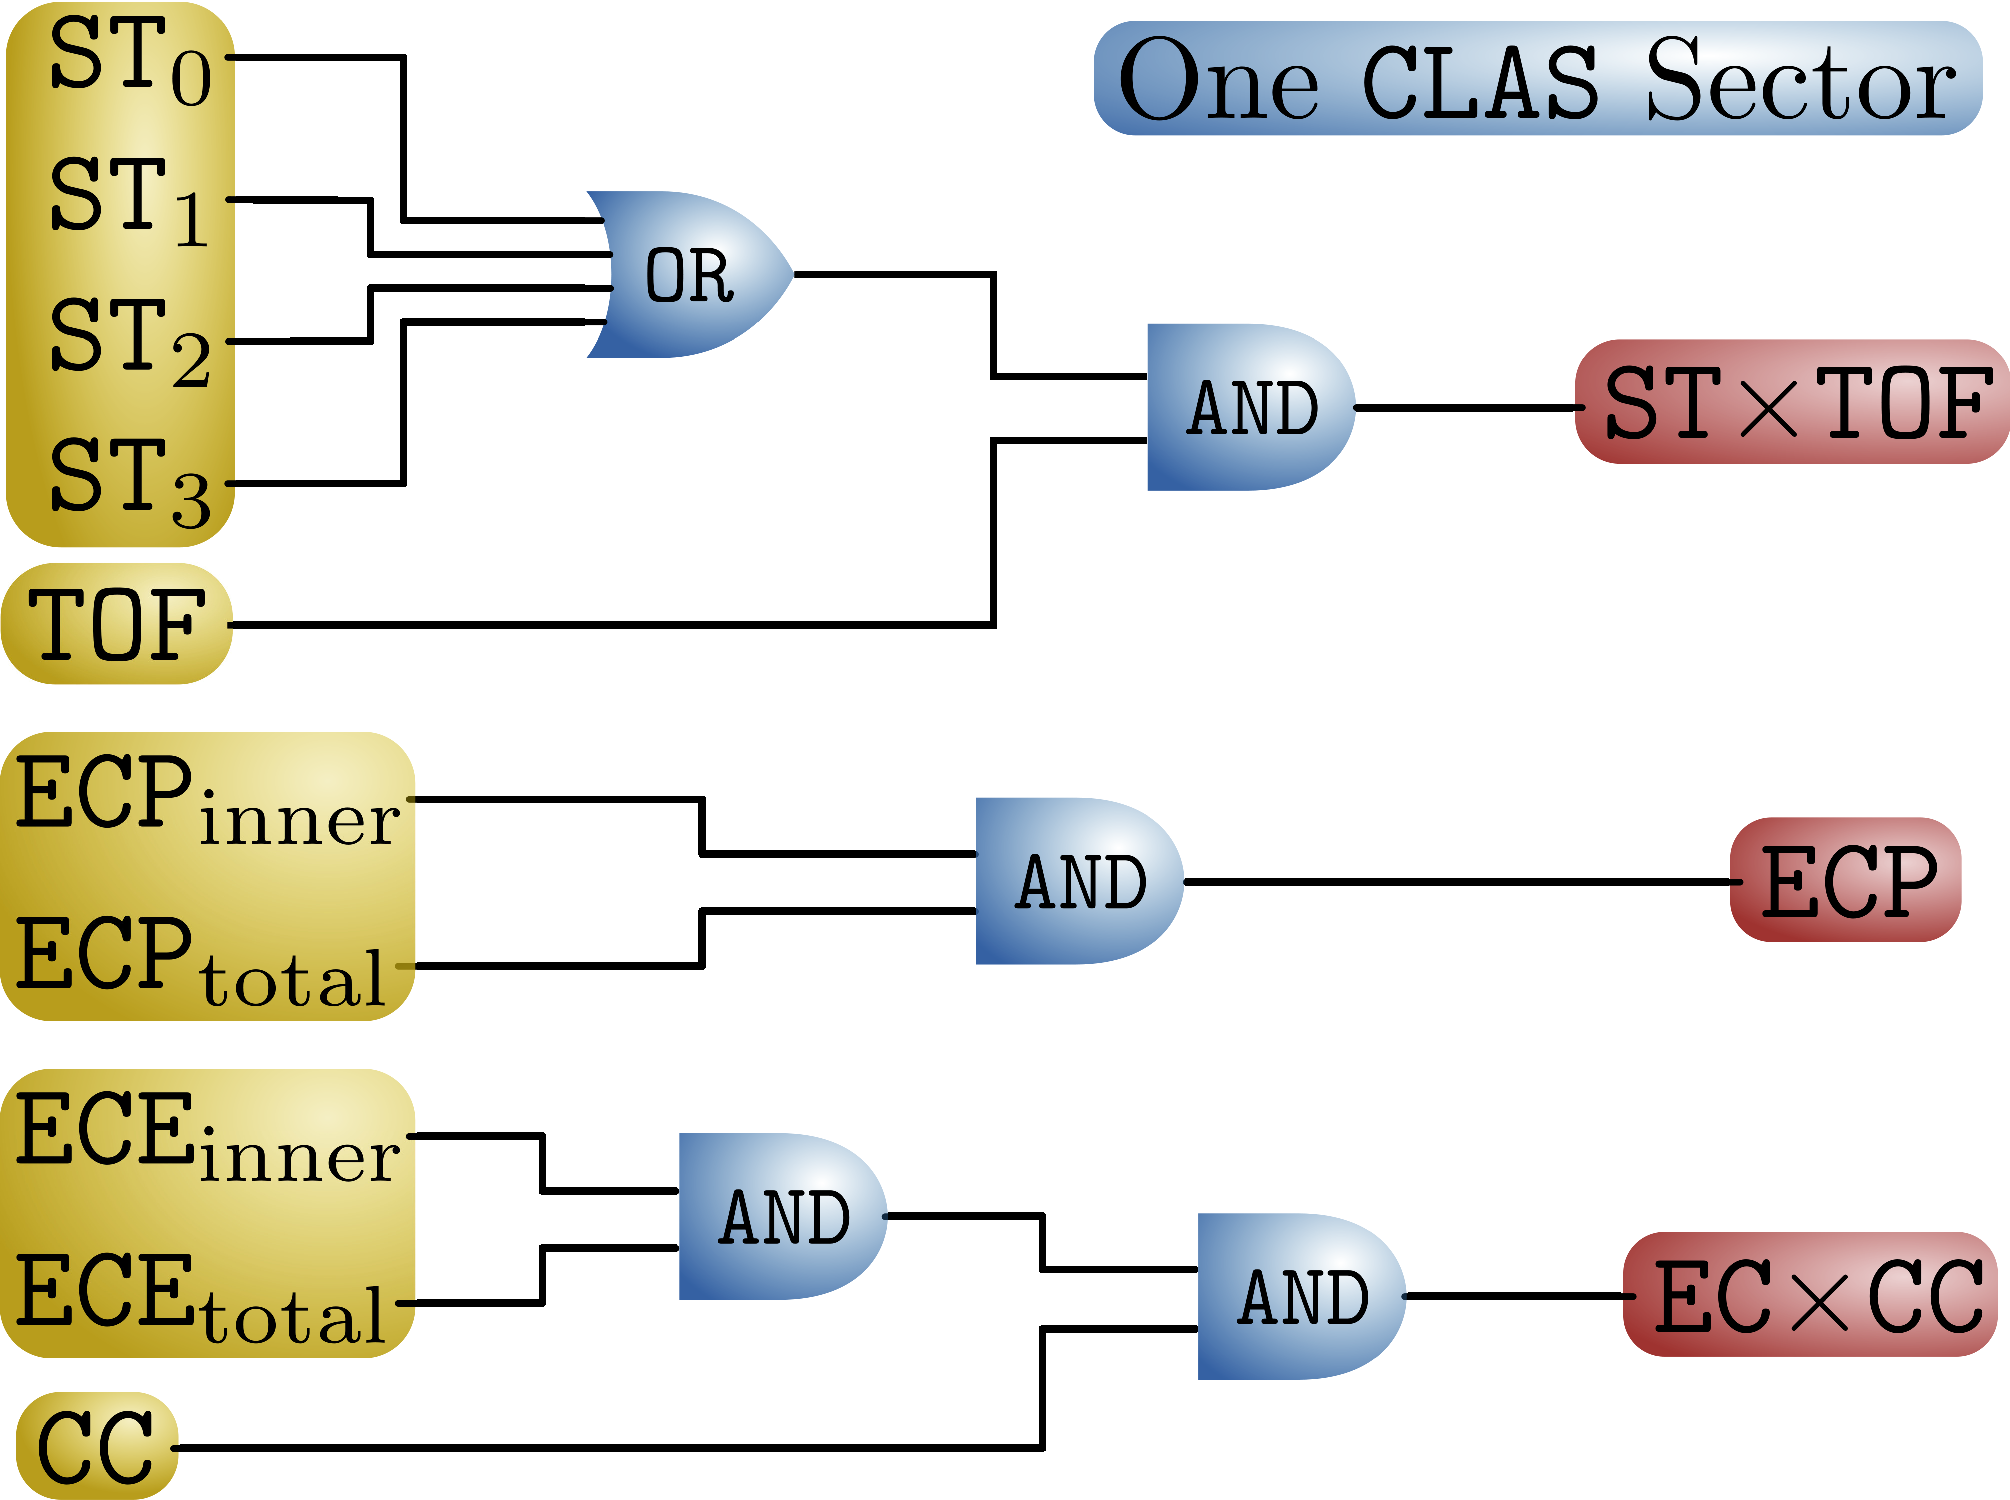
\includegraphics[width=0.8\figwidth]{\figures/hall-b/trigger_sector.pdf}
%\caption[Trigger Logic - One Sector]{\label{fig:clas.daq.trigsec}{\coloronline}Trigger logic for one of the six sectors of \abbr{CLAS}. The \abbr{ST$\times$TOF} signal is a coincidence between any of the four start counter \abbr{TDC} signals (numbered from 0 to 3) and any of the 57 \abbr{TOF} \abbr{TDC} signals. The \abbr{ECE}$_\mathrm{inner}$ and \abbr{ECE}$_{\mathrm{total}}$ are the \emph{electron}-threshold \abbr{EC} signals for the energy deposited in the \emph{inner} layer and in \emph{all} layers. These are combined with a \abbr{CC} signal to produce the \abbr{EC$\times$CC} trigger for this sector. The \abbr{ECP} trigger signal is the \emph{photon}-threshold \abbr{EC} signal. These trigger signals are discussed further in Sec.~\ref{sec:data.trig}.}
%\end{center}\end{figure}
